\chapter{Теоритический раздел}

RISC-V является открытым современным набором команд, который может использоваться для построения как микроконтроллеров, так и высокопроизводительных микропроцессоров. В связи с такой широкой областью применения в систему команд введена вариативность. Таким образом, термин RISC-V фактически является названием для семейства различных систем команд, которые строятся вокруг базового набора команд, путем внесения в него различных расширений.

В данной работе исследуется набор команд RV32I, который включает в себя основные команды 32-битной целочисленной арифметики кроме умножения и деления. В рамках данного набора команд мы не будем рассматривать системные команды, связанные с таймерами, системными регистрами, управлением привилегиями, прерываниями и исключениями.

\section{Архитектура набора команд RV32I}

В настоящем разделе описывается архитектура набора команд, то есть архитектура абстрактной вычислительной машины с точки зрения набора команд без связи с конкретной аппаратной реализацией.

\subsection{Регистровая модель}

Набор команд RV32I предполагает использование 32 регистров общего назначения x0-x31 размером в 32 бита каждый и регистр pc, хранящего адрес следующей команды. Все регистры общего назначения равноправны, в любой команде могут использоваться любые из регистров. Регистр pc не может использоваться в командах.

\subsection{Модель памяти}

Архитектура RV32I предполагает плоское линейное 32-х битное адресное пространство. Минимальной адресуемой единицей информации является 1 байт. Используется порядок байтов от младшего к старшему (Little Endian), то есть, младший байт 32-х битного слова находится по младшему адресу (по смещению 0). Отсутствует разделение на адресные пространства команд, данных и ввода-вывода. Распределение областей памяти между различными устройствами (ОЗУ, ПЗУ, устройства ввода-вывода) определяется реализацией.

\subsection{Система команд}

Большая часть команд RV32I является трехадресными, выполняющими операции над двумя заданными явно операндами, и сохраняющими результат в регистре. Операндами могут являться регистры или константы, явно заданные в коде команды. Операнды всех команд (кроме команды auipc) задаются явно.

Архитектура RV32I, как и большая часть RISC-архитектур, предполагает разделение команд на команды доступа к памяти (чтение данных из памяти в регистр или запись данных из регистра в память) и команды обработки данных в регистрах.

Таким образом, команды RV32I можно разделить на следующие категории:

\begin{enumerate}
	\item Команды обработки данных
	\begin{enumerate}
		\item Арифметические и логические команды
		\item Команды сравнения
		\item Команды сдвига
		\item Команды формирования значения в старшей части регистра
	\end{enumerate}
	\item Команды передачи управления
	\begin{enumerate}
		\item Команды безусловного перехода с сохранением адреса возврата
		\item Команды условного перехода
	\end{enumerate}
	\item Команды доступа к памяти
	\begin{enumerate}
		\item Команды загрузки
		\item Команды сохранения
	\end{enumerate}
	\item Системные команды
\end{enumerate}

\chapter{Экспериментальный раздел}

\section{Исследование программы}

\subsection{Исходный код программы}

\begin{lstlisting}
		.section .text
		.globl _start;
		len = 8      # Размер массива
		enroll = 1   # Количество обрабатываемых элементов за одну итерацию
		elem_sz = 4  # Размер одного элемента массива
	
_start:
		la x1, _x
		addi x20, x1, elem_sz*(len-1) # Адрес последнего элемента
lp:
		lw x2, 0(x1)
		add x31, x31, x2 \#!
		addi x1, x1, elem_sz*enroll
		bne x1, x20, lp
		addi x31, x31, 1
lp2: 	j lp2

		.section .data
_x:     .4byte 0x1
		.4byte 0x2
		.4byte 0x3
		.4byte 0x4
		.4byte 0x5
		.4byte 0x6
		.4byte 0x7
		.4byte 0x8
\end{lstlisting}

\pagebreak

\subsection{Дизассемблированный листинг}

\begin{lstlisting}
Disassembly of section .text:

80000000 <_start>:
80000000:       00000097                auipc   x1,0x0
80000004:       02408093                addi    x1,x1,36 # 80000024 <_x>
80000008:       01c08a13                addi    x20,x1,28

8000000c <lp>:
8000000c:       0000a103                lw      x2,0(x1)
80000010:       002f8fb3                add     x31,x31,x2
80000014:       00408093                addi    x1,x1,4
80000018:       ff409ae3                bne     x1,x20,8000000c <lp>
8000001c:       001f8f93                addi    x31,x31,1

80000020 <lp2>:
80000020:       0000006f                jal     x0,80000020 <lp2>

Disassembly of section .data:

80000024 <_x>:
80000024:       0001                    c.addi  x0,0
80000026:       0000                    unimp
80000028:       0002                    0x2
8000002a:       0000                    unimp
8000002c:       00000003                lb      x0,0(x0) # 0 <enroll-0x1>
80000030:       0004                    c.addi4spn      x9,x2,0
80000032:       0000                    unimp
80000034:       0005                    c.addi  x0,1
80000036:       0000                    unimp
80000038:       0006                    0x6
8000003a:       0000                    unimp
8000003c:       00000007                0x7
80000040:       0008                    c.addi4spn      x10,x2,0
\end{lstlisting}

\pagebreak

\subsection{Псевдокод}

\begin{lstlisting}[language=C,caption=Эквивалентный код на С.]
#define len 	8
#define enroll 	1
#define elem_sz 4

int _x[] = { 1, 2, 3, 4, 5, 6, 7, 8 };

void _start()
{
	int *x1 = &_x;
	int *x20 = x1 + elem_si * (len - 1);
	int x31 = 0;
	
	do
	{
		int x2 = *x1;
		x31 += x2;
		x1 += elem_sz * enroll;
	}
	while (x1 != x20);
	
	x31++;
	
	while (1) {}
}
\end{lstlisting}

\pagebreak

\paragraph{Задание 2.}

Получить снимок экрана, содержащий временную диаграмму выполнения стадий выборки и диспетчеризации команды с указанным адресом.

Адрес команды: 80000014, номер итерации: 1.

\begin{figure}
	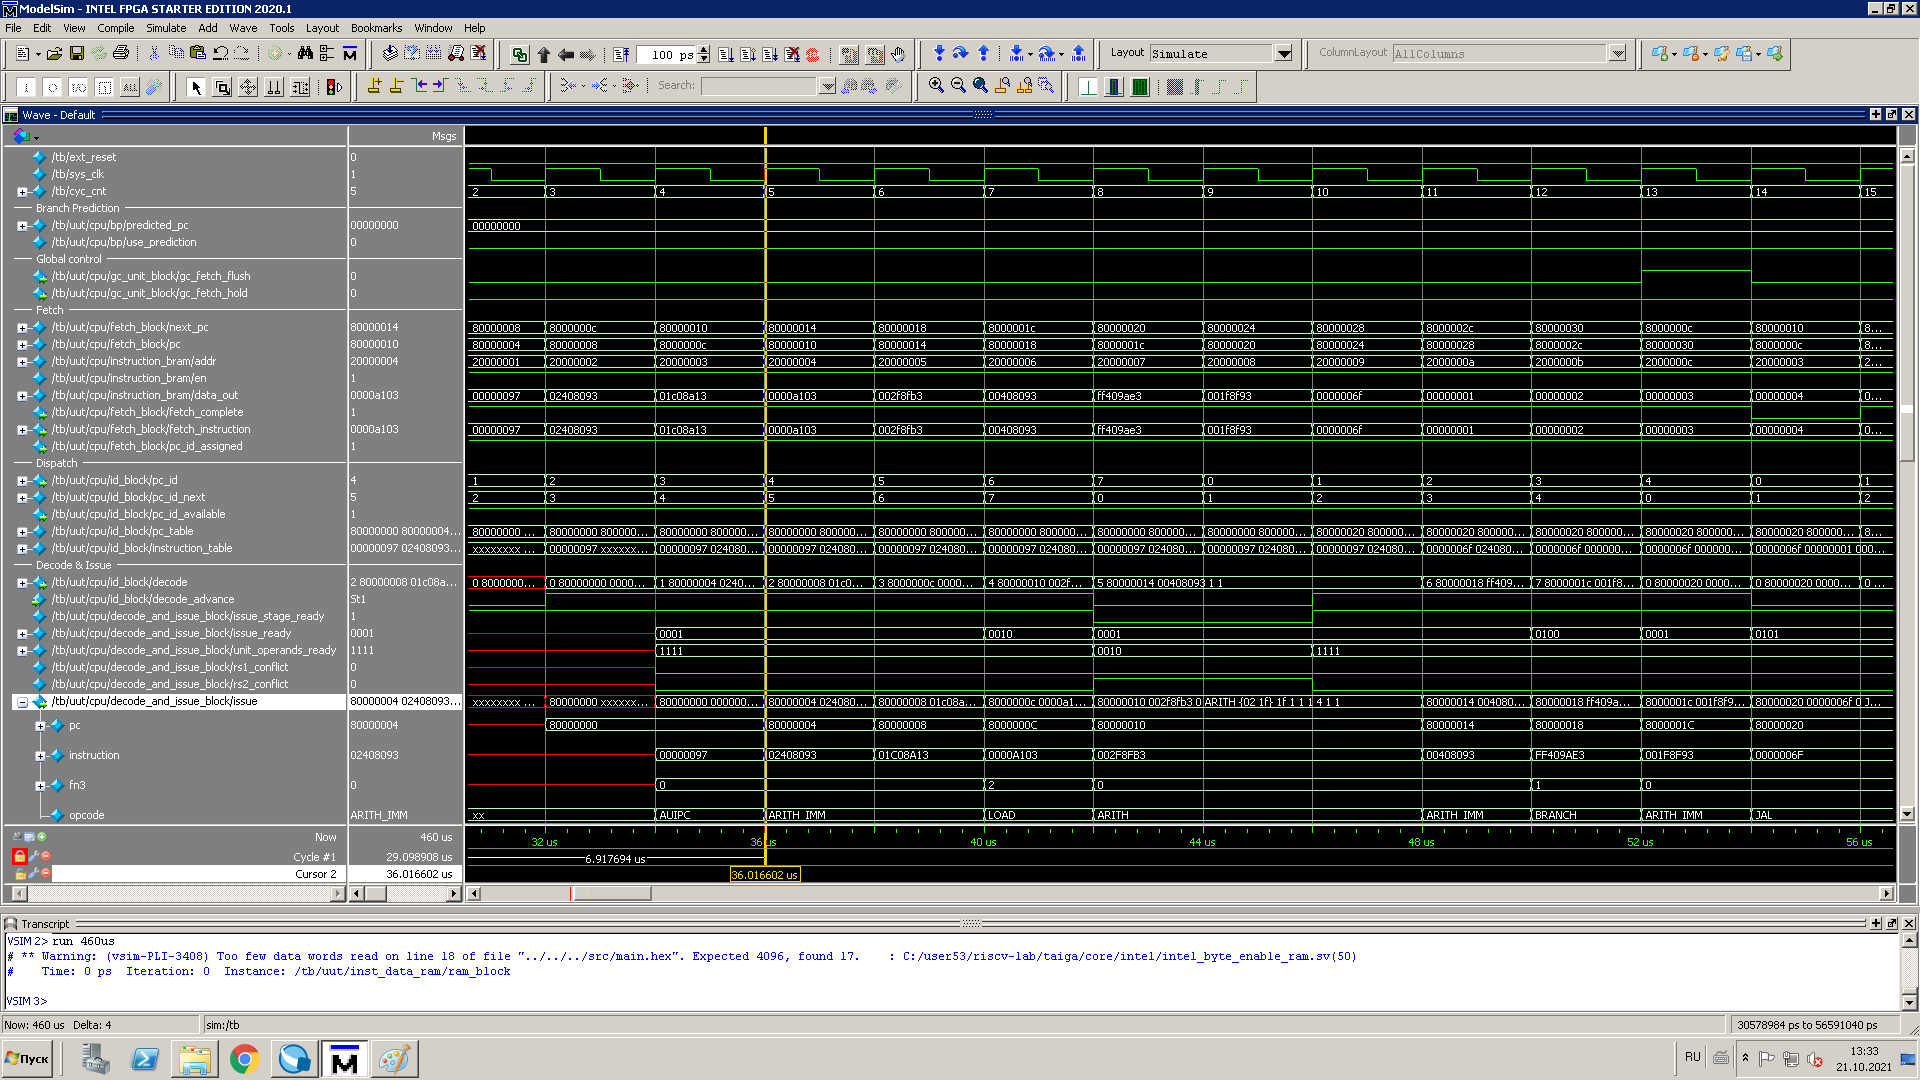
\includegraphics[width=\textwidth,height=\textheight,keepaspectratio]{img/img1.png}
	\caption{Скриншот для задания 2}
\end{figure}

\clearpage

\paragraph{Задание 3.}

Получить снимок экрана, содержащий временную диаграмму выполнения стадии декодирования и планирования на выполнение команды с указанным адресом.

Адрес команды: 80000020, номер итерации: 1.

\begin{figure}
	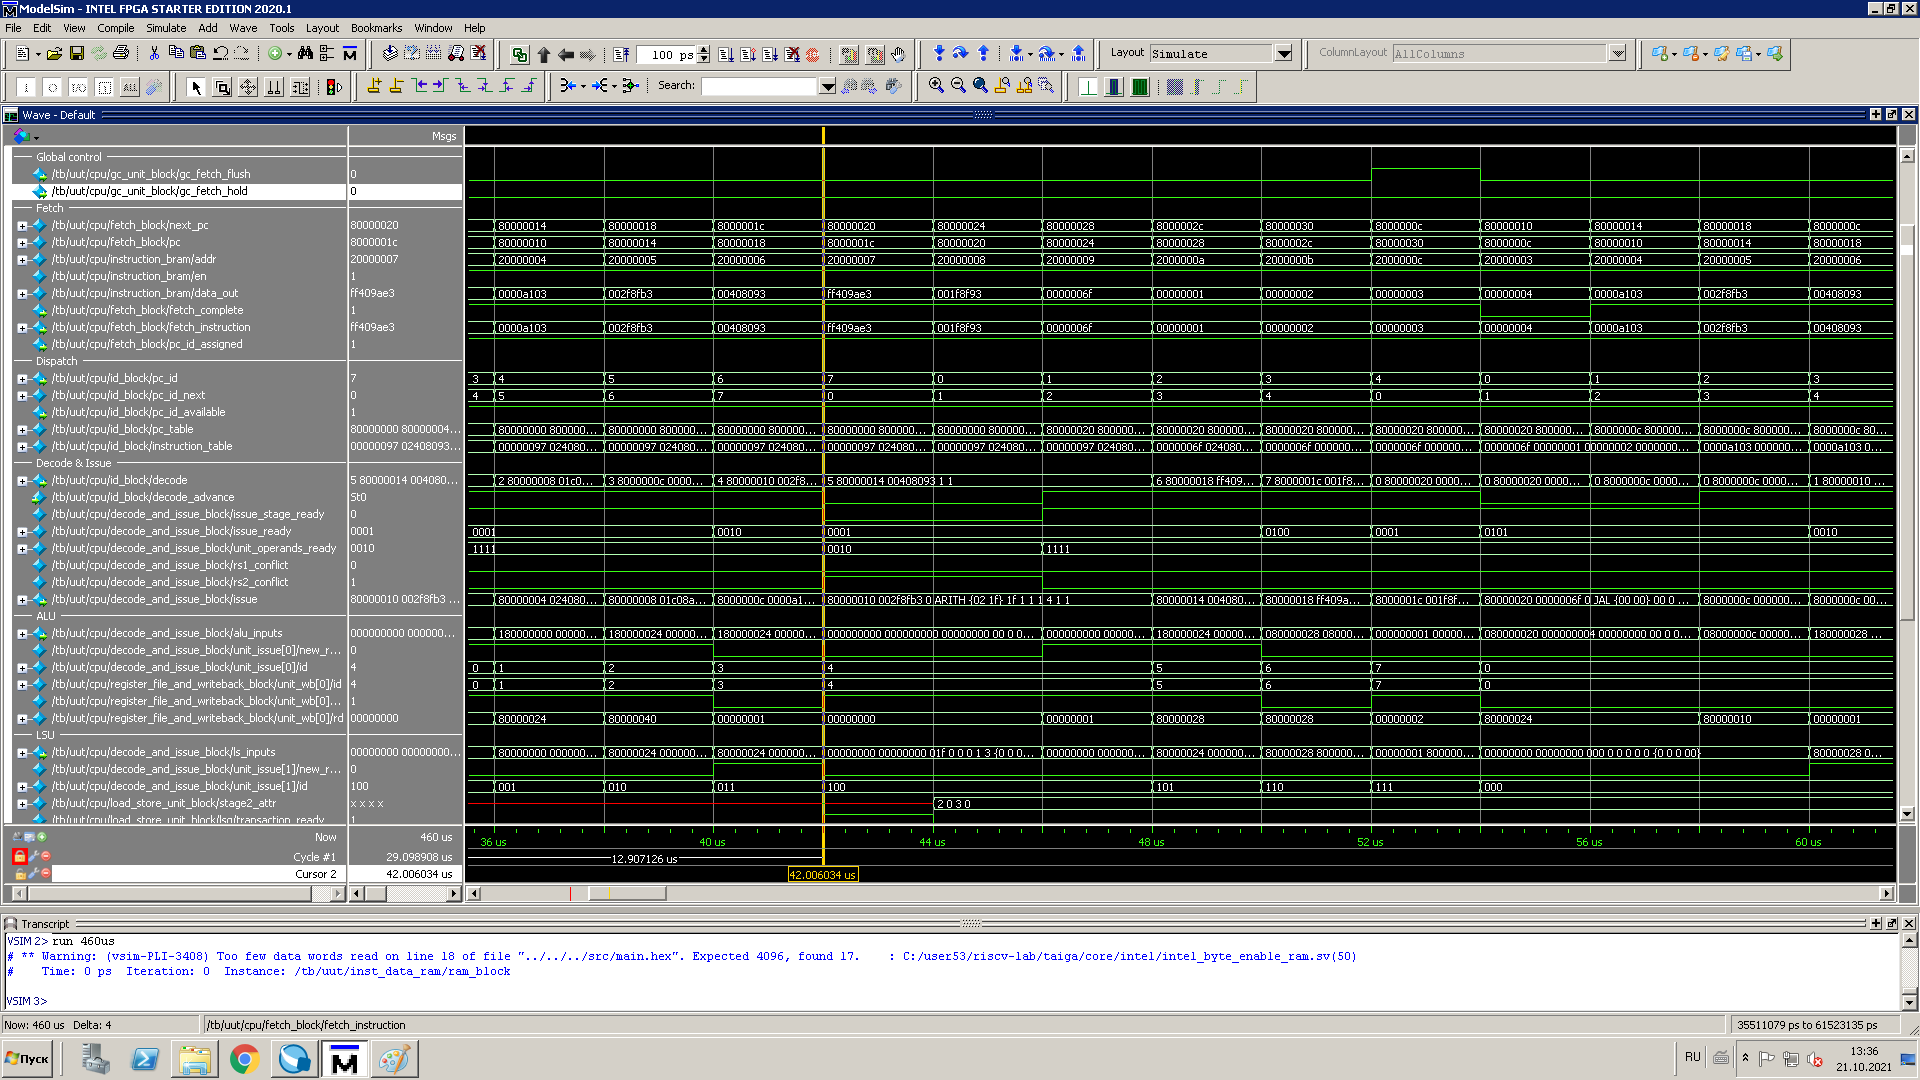
\includegraphics[width=\textwidth,height=\textheight,keepaspectratio]{img/img2.png}
	\caption{Скриншот для задания 3}
\end{figure}

\clearpage

\paragraph{Задание 4.}

Получить снимок экрана, содержащий временную диаграмму выполнения стадии выполнения команды с указанным адресом.

Адрес команды: 80000008.

\begin{figure}
	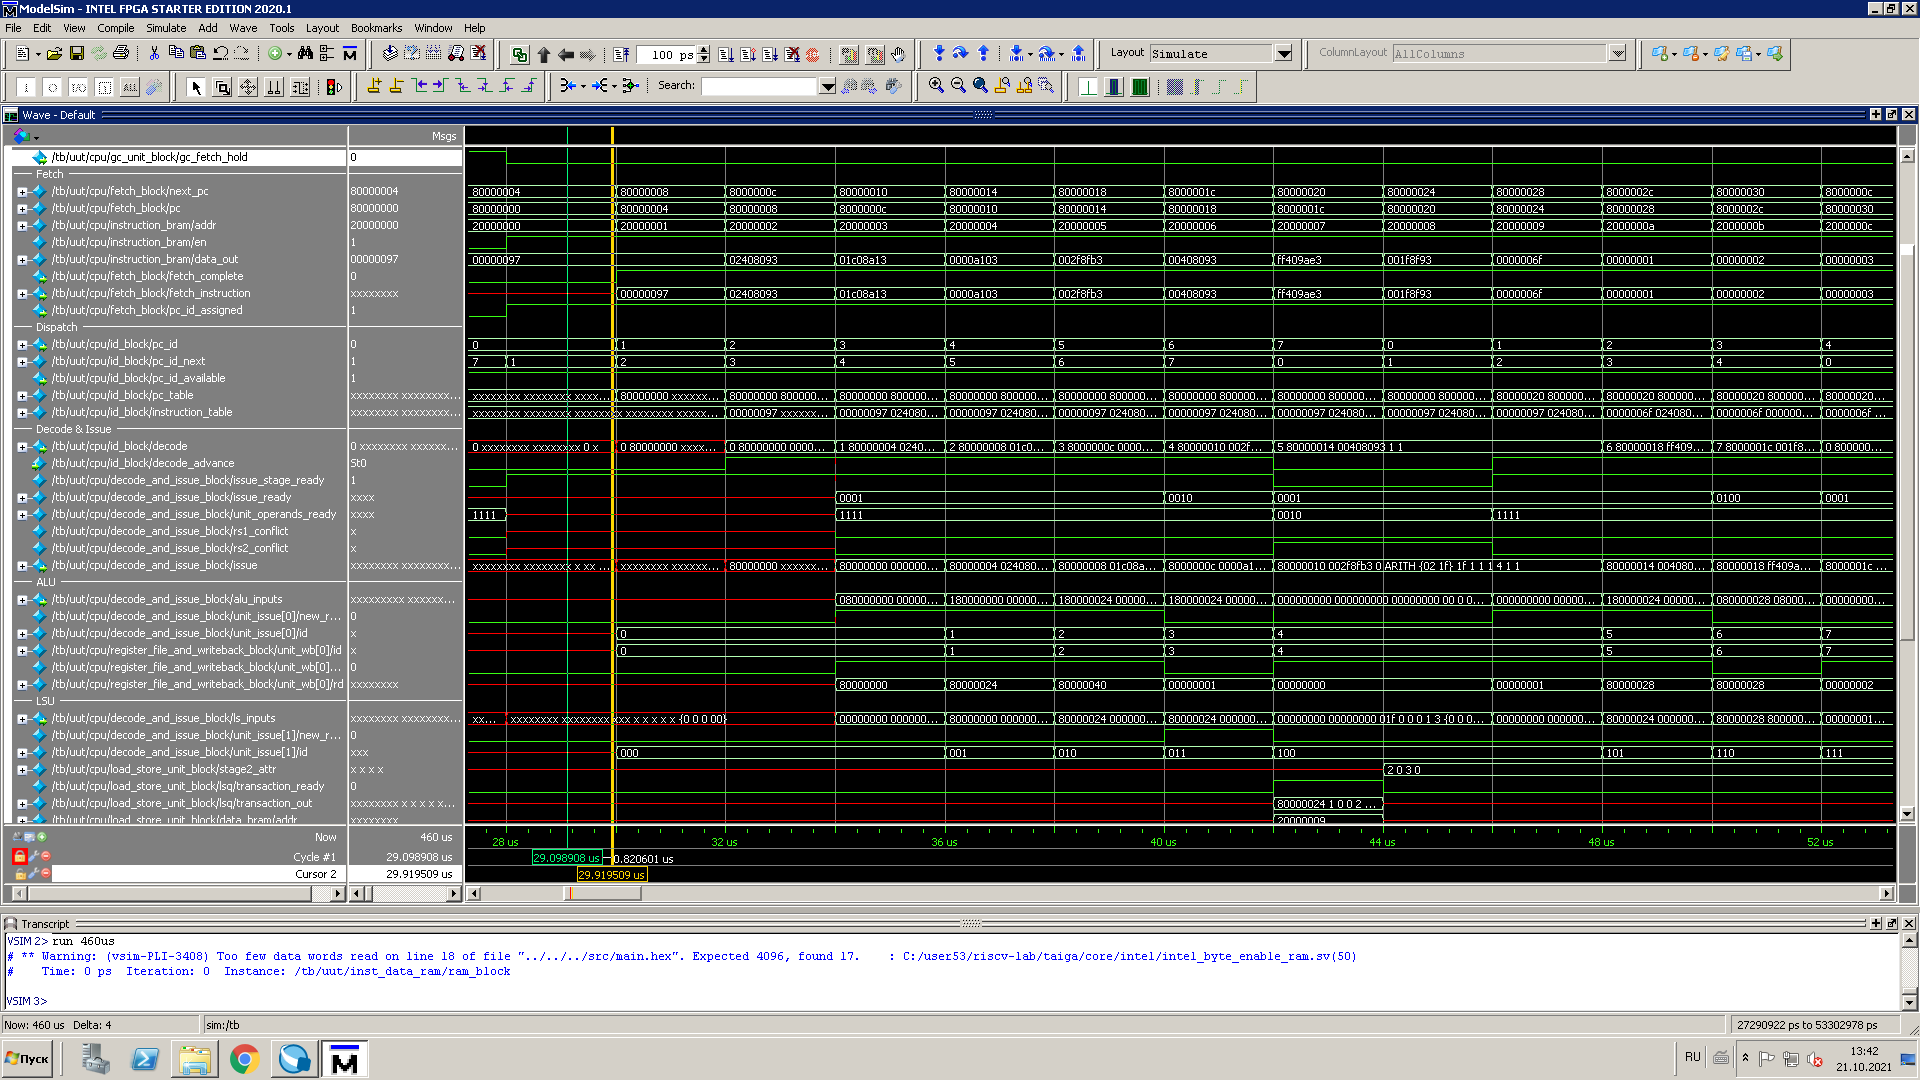
\includegraphics[width=\textwidth,height=\textheight,keepaspectratio]{img/img3.png}
	\caption{Скриншот для задания 4}
\end{figure}

\pagebreak

\subsection{Трасса работы программы}

\begin{figure}
	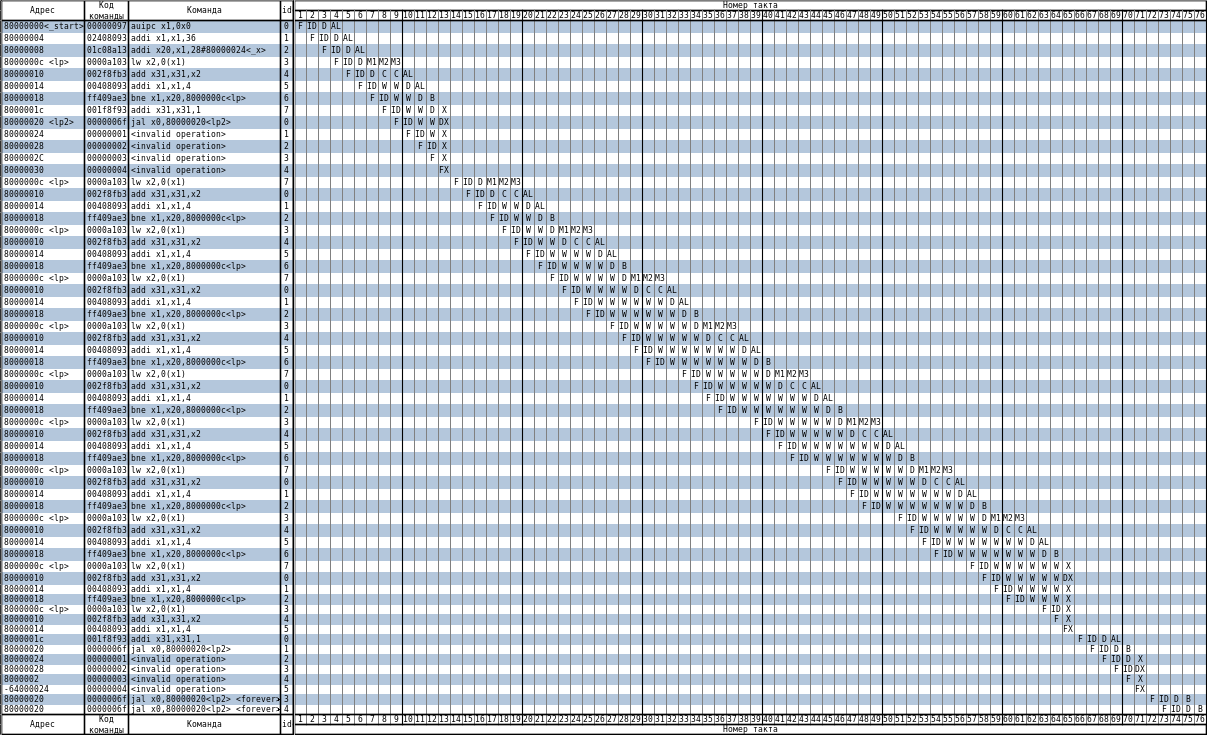
\includegraphics[width=\linewidth]{img/init.png}
\end{figure}

\subsection{Выводы об эффективности}

{\sloppy
Из рассмотрения трассы видно, что выполнение программы до окончания команды \verb|addi x31,x31,1| заняло 69 тактов (1-69). Из них, в течение 23 тактов (7, 8, 13-15, 17, 18, 23, 24, 29, 30, 35, 36, 41, 42, 47, 48, 53, 54, 60, 65-67) не происходило планирование на выполнение новых команд, то есть, 50\% времени было потрачено не эффективно из-за ошибок предсказания ветвлений и конфликтов на конвейере.\par}

{\sloppy
Для оптимизации данной программы можно поменять местами команды на строках 12 и 13. После этого конвеер сможет приступить к обработке следующей команды после планирования \verb|lw x2,0(x1)|.\par}

\pagebreak

\section{Оптимизация программы}

\subsection{Исходный код оптимизированной программы}

\begin{lstlisting}
		.section .text
		.globl _start;
		len = 8      # Размер массива
		enroll = 1   # Количество обрабатываемых элементов за одну итерацию
		elem_sz = 4  # Размер одного элемента массива

_start:
		la x1, _x
		addi x20, x1, elem_sz*(len-1) # Адрес последнего элемента
lp:
		lw x2, 0(x1)
		addi x1, x1, elem_sz*enroll
		add x31, x31, x2
		bne x1, x20, lp
		addi x31, x31, 1
lp2: 	j lp2

		.section .data
_x:     .4byte 0x1
		.4byte 0x2
		.4byte 0x3
		.4byte 0x4
		.4byte 0x5
		.4byte 0x6
		.4byte 0x7
		.4byte 0x8
\end{lstlisting}

\pagebreak

\subsection{Дизассемблированный листинг оптимизированной программы}

\begin{lstlisting}
	Disassembly of section .text:
	
	80000000 <_start>:
	80000000:       00000097                auipc   x1,0x0
	80000004:       02408093                addi    x1,x1,36 # 80000024 <_x>
	80000008:       01c08a13                addi    x20,x1,28
	
	8000000c <lp>:
	8000000c:       0000a103                lw      x2,0(x1)
	80000010:       00408093                addi    x1,x1,4
	80000014:       002f8fb3                add     x31,x31,x2
	80000018:       ff409ae3                bne     x1,x20,8000000c <lp>
	8000001c:       001f8f93                addi    x31,x31,1
	
	80000020 <lp2>:
	80000020:       0000006f                jal     x0,80000020 <lp2>
	
	Disassembly of section .data:
	
	80000024 <_x>:
	80000024:       0001                    c.addi  x0,0
	80000026:       0000                    unimp
	80000028:       0002                    0x2
	8000002a:       0000                    unimp
	8000002c:       00000003                lb      x0,0(x0) # 0 <enroll-0x1>
	80000030:       0004                    c.addi4spn      x9,x2,0
	80000032:       0000                    unimp
	80000034:       0005                    c.addi  x0,1
	80000036:       0000                    unimp
	80000038:       0006                    0x6
	8000003a:       0000                    unimp
	8000003c:       00000007                0x7
	80000040:       0008                    c.addi4spn      x10,x2,0
\end{lstlisting}

\pagebreak

\subsection{Трасса работы оптимизированной программы}

\begin{figure}
	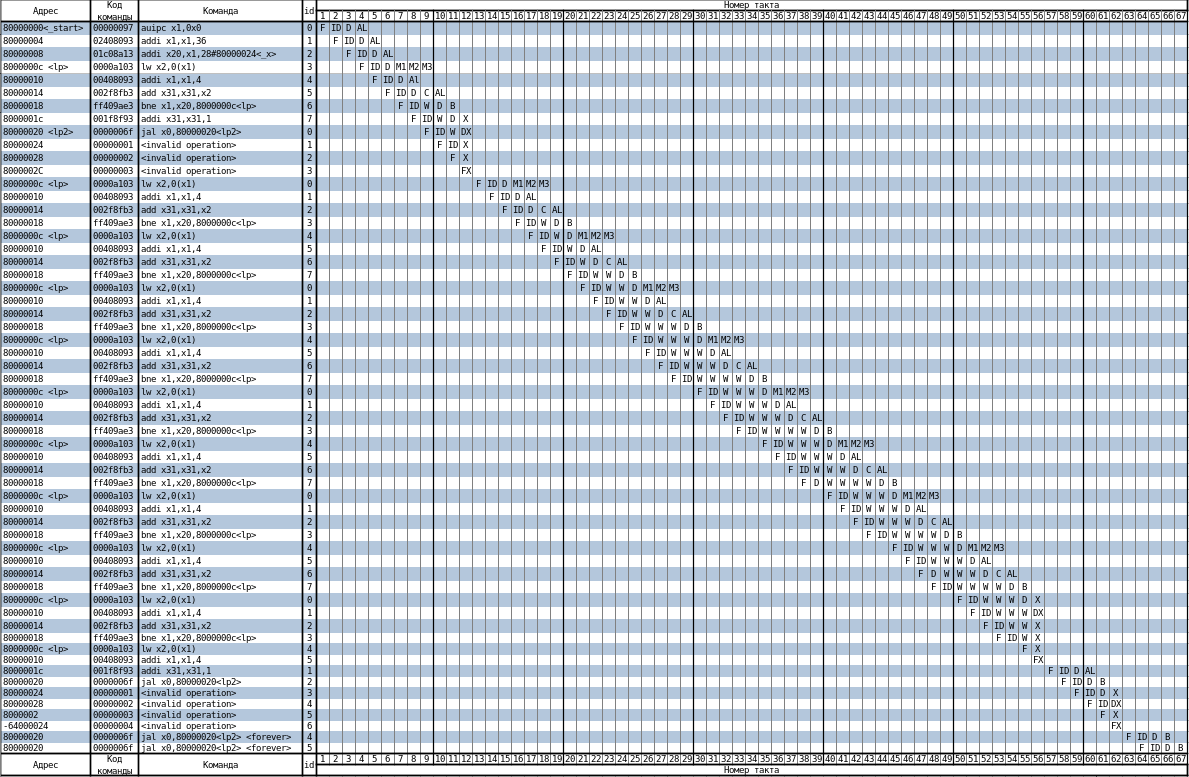
\includegraphics[width=\linewidth]{img/opt.png}
\end{figure}

\subsection{Выводы}

Выполнение оптимизированной программы до окончания каманды \verb|addi x31,x31,1| заняло 60 тактов, что на 13\% быстрее неоптимизированной программы.

Рассмотрев трассу работы оптимизированной программы, можно обнаружить, что планирование на выполнение новых команд происходило только 13 тактов (8, 12, 13, 17, 22, 27, 32, 37, 42, 47, 52, 56, 57).



